%% Obhajoba diplomové práce — Detekce anomálií v časových řadách spotřeby vody
%% Bc. Ondřej Černý, FIT ČVUT
%% Šablona: ctufit-presentation (beamer)
%%
%% Kompilace: xelatex -> (biber) -> xelatex -> xelatex
%%
%% POZNÁMKA K OBRÁZKŮM:
%% Slajdy s výsledky odkazují na PNG z vaší práce (složka images/).
%% Zkopírujte složku images/ z repozitáře práce vedle tohoto .tex souboru,
%% nebo upravte \graphicspath níže.

% arara: xelatex
% arara: xelatex

%%%%%%%%%%%%%%%%%%%%%%%%%%%%%%%%%%%%%%%%%
% CLASS OPTIONS
% language: czech/english/slovak
% nobg: removes lion background image
% nonumber: removes page numbers from the sidebar
% colour: orange (default) or blue
%%%%%%%%%%%%%%%%%%%%%%%%%%%%%%%%%%%%%%%%%
\documentclass[czech,blue]{ctufit-presentation}

\usepackage{tikz}
\usetikzlibrary{arrows.meta,positioning,fit,backgrounds}
\usepackage{booktabs}

% Cesta k obrázkům z práce (uprav podle umístění složky images/)
\graphicspath{{images/}{./}}

\ctufittitle{Detekce anomálií v časových řadách \\[2pt] spotřeby vody}
\ctufitauthor{Autor: Bc.~Ondřej Černý \\[2pt] Vedoucí: doc.\,Ing.\,Kamil Dedecius,\,Ph.D.}
%\ctufitinstitute{FIT ČVUT}

% Barvy pro zvýraznění v tabulkách / schématech
\definecolor{accent}{RGB}{0,122,194}
\definecolor{good}{RGB}{0,140,72}
\definecolor{warn}{RGB}{200,60,40}

\begin{document}

%=============================================================================================
% TITULNÍ SLAJD
%=============================================================================================
\begin{frame}[plain,t]
	\titlepage
\end{frame}

% (Outline slajd záměrně vynechán — viz pokyn vedoucího.)

%=============================================================================================
\section{Motivace}
%=============================================================================================
\begin{frame}
	\frametitle{Motivace a cíle}
	\begin{exampleblock}{Motivace}
		\begin{itemize}
			\item Detekce anomalií na datech z vodoměrů od Softlink s.r.o.
			\item Dnes: pevné prahy = neadaptivní
		\end{itemize}
	\end{exampleblock}
	\vspace{0.2em}
	\begin{block}{\textcolor{black}{Cíle práce}}
		\begin{enumerate}
			\item Výběr vhodných statistických nebo ML metod
			\item Implementace daných metod na datech Softlinku
			\item Diskuze výsledků
		\end{enumerate}
	\end{block}
	\vspace{0.2em}
	\begin{center}
		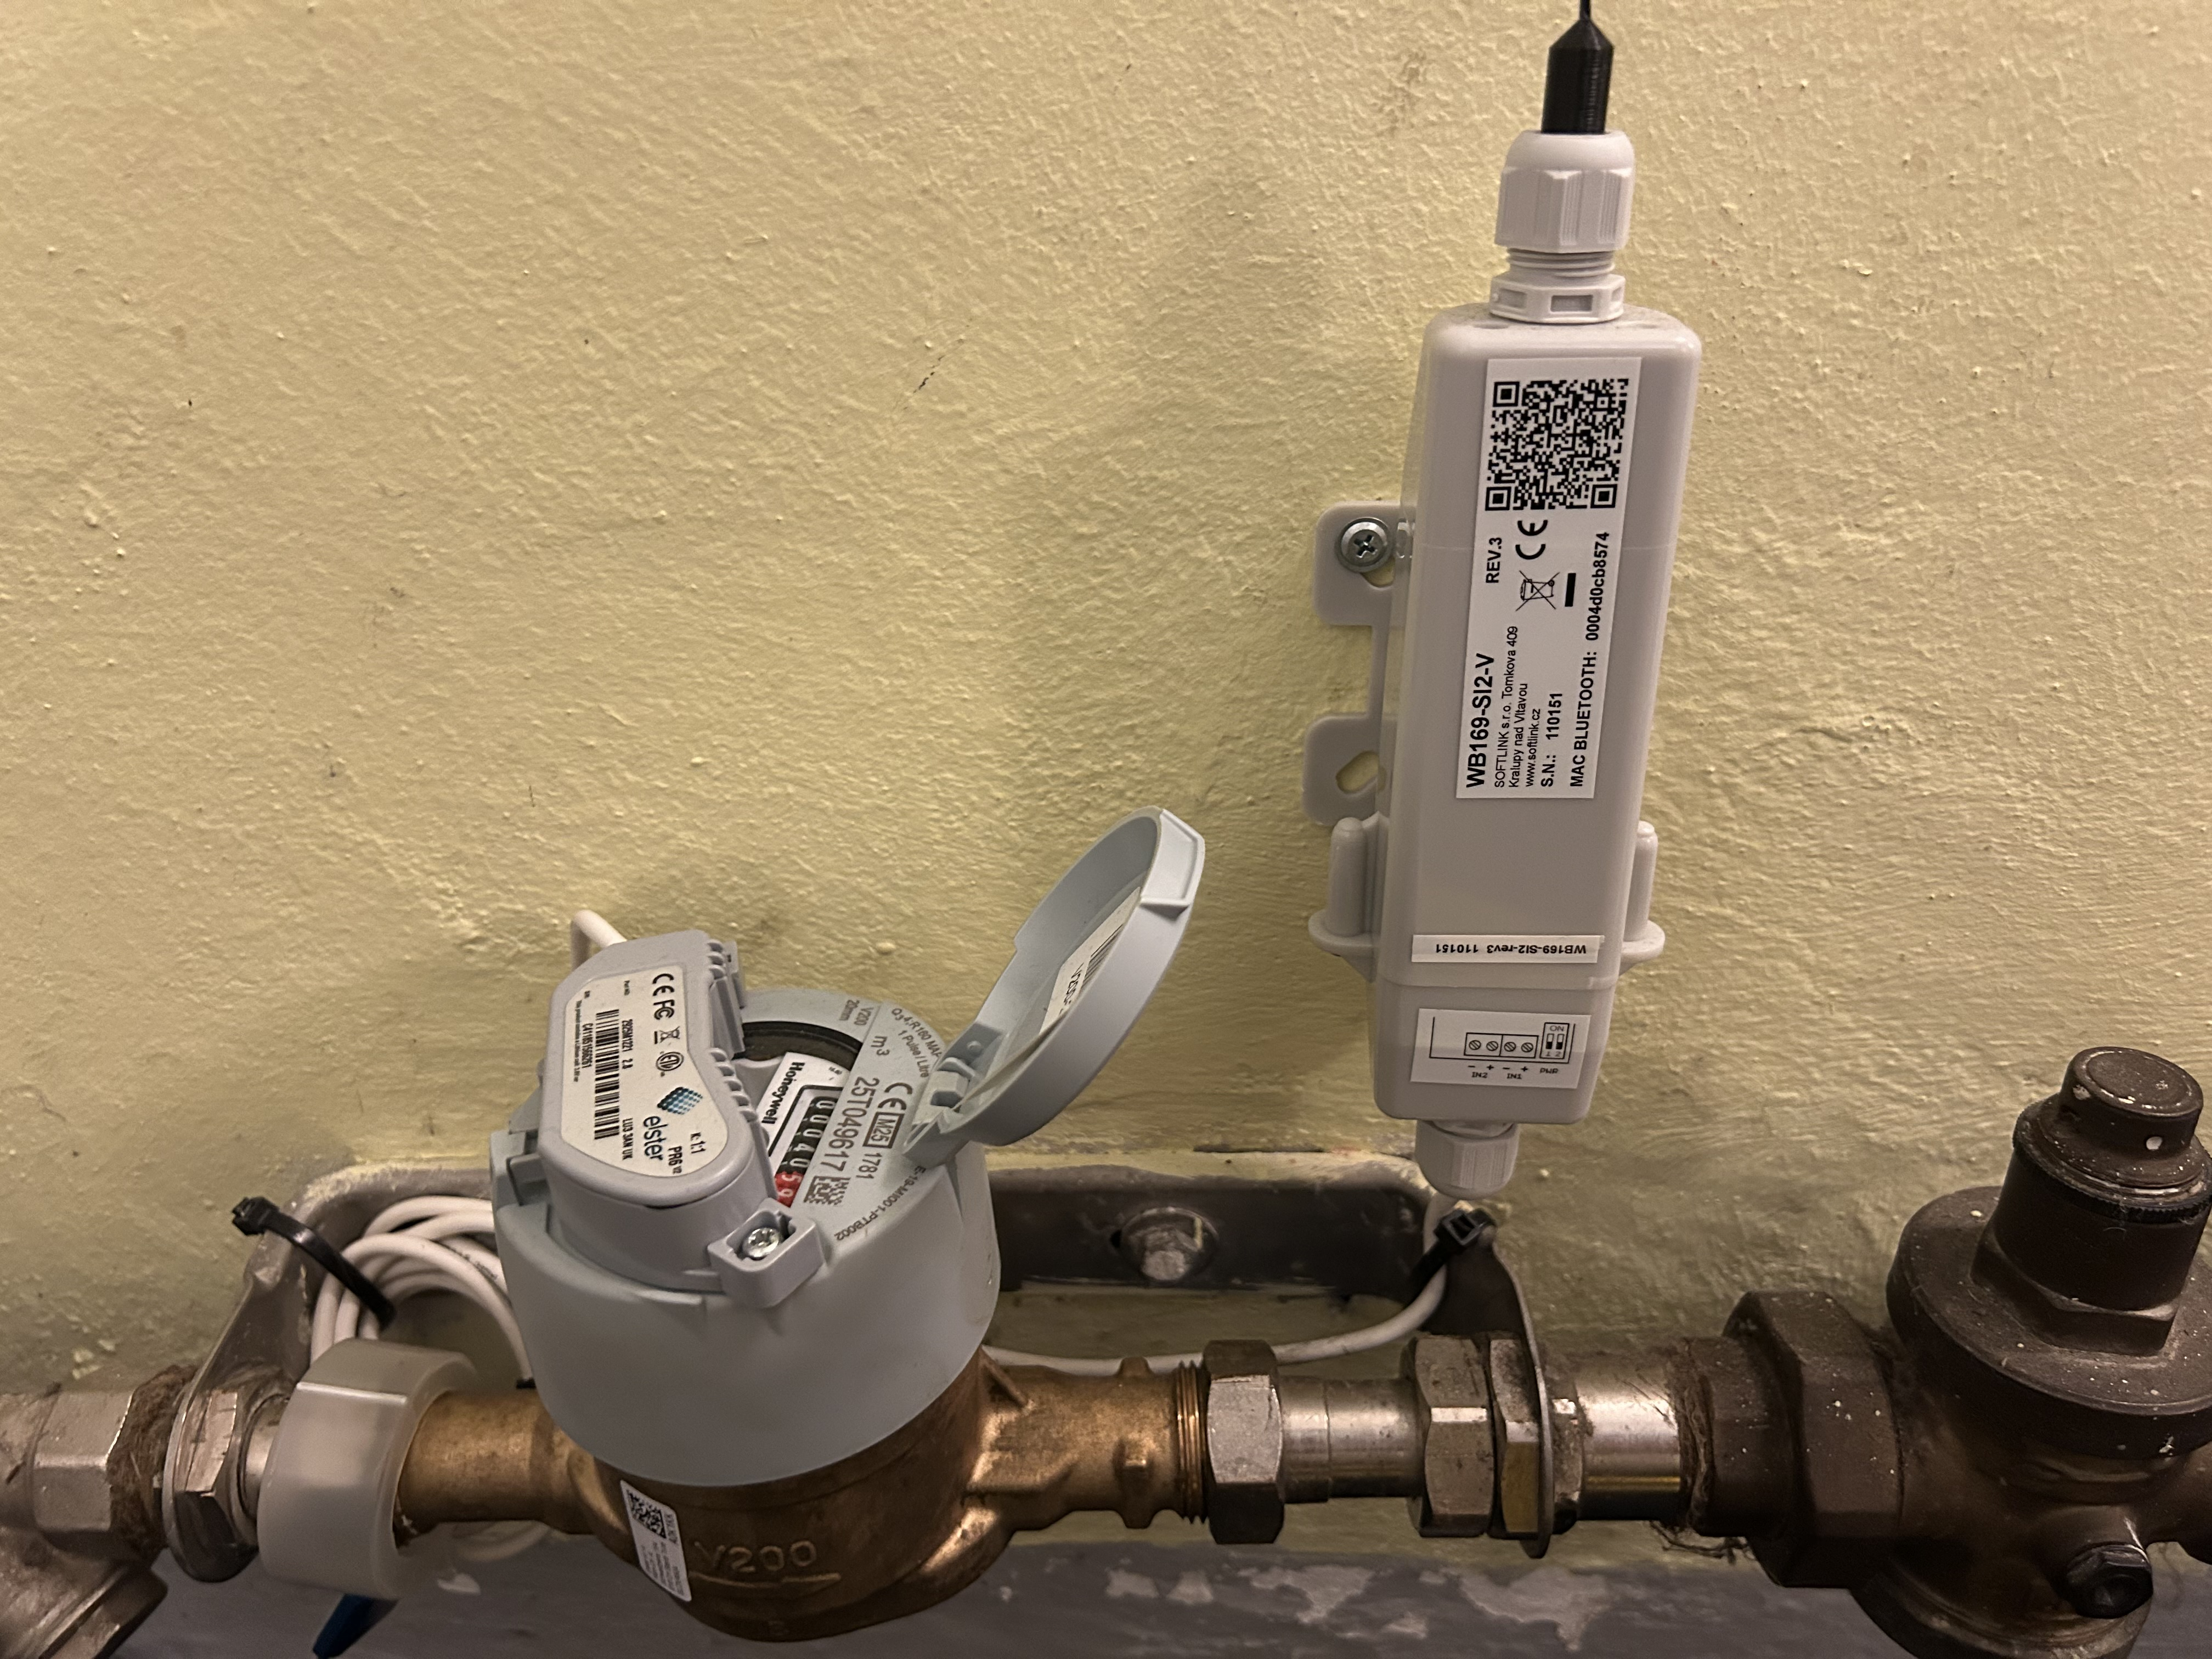
\includegraphics[width=4.5cm,keepaspectratio]{./images/sensor_doma.jpg}
	\end{center}
\end{frame}

%=============================================================================================
\section{Data}
%=============================================================================================
\begin{frame}
	\frametitle{Data od Softlink s.r.o.}
	\begin{itemize}
		\item \textbf{27\,000}+ senzorů \\ {\small (průmyslové budovy, sklady, obytné budovy, ...)}
		\item \textbf{618 mil.} hodnot měření = posledních 5 let
		\item $\texttt{Diff}_t = \texttt{Hodnota}_t - \texttt{Hodnota}_{t-1}$
	\end{itemize}
	\vspace{0.4em}
	\begin{tabular}{|c|c|c|c|}
		\hline
		\textbf{Id} & \textbf{Timestamp} & \textbf{Hodnota} & \textbf{Diff}\\ \hline
		2077 & 2024-07-01 08:00:00 & 9.220 & - \\ \hline
		2077 & 2024-07-01 09:00:00 & 11.460 & 2.240\\ \hline
		2077 & 2024-07-01 10:00:00 & 14.550 & 3.090\\ \hline
	\end{tabular}
	
	\vspace{0.4em}
	\begin{alertblock}{Omezení}
		\begin{itemize}
			\item Nespecifikované periody měření
			\item Žádná data o objektech (pouze \texttt{id})
		\end{itemize}
	\end{alertblock}			
\end{frame}

\begin{plainFrame}
	\includegraphics[width=\paperwidth,height=\paperheight,keepaspectratio]{./images/actuals_only.png}
\end{plainFrame}

%=============================================================================================
\section{Přístup}
%=============================================================================================
\begin{frame}
	\frametitle{Implementace: Detekce z predikčních reziduí}
	\begin{columns}[T]
		\begin{column}{0.55\textwidth}
			\begin{itemize}
				\item Jeden model na jeden senzor
				\item Predikční modely
				\begin{itemize}
					\item Jednokrokové
					\item Univarietní - Diff
					\item Dva typy: Strukturální modely a GRU NN
				\end{itemize}
				\item Stejný princip detekce
			\end{itemize}
		\end{column}
		\begin{column}{0.45\textwidth}
			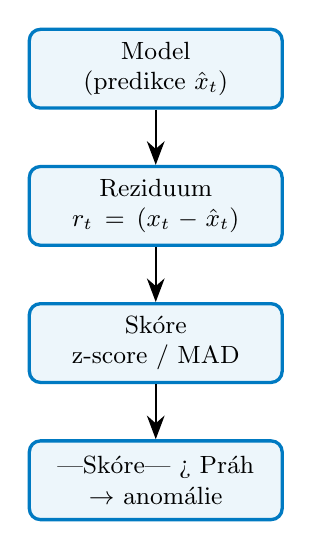
\begin{tikzpicture}[
				node distance=7mm,
				box/.style={rounded corners,draw=accent,very thick,fill=accent!7,
					align=center,minimum height=10mm,inner sep=3pt,font=\small,
					text width=3cm},
				arr/.style={-{Stealth[length=3mm]},thick}]
				\node[box] (model) {Model\\(predikce $\hat{x}_t$)};
				\node[box,below=of model] (res) {Reziduum\\$r_t=(x_t-\hat{x}_t)$};
				\node[box,below=of res] (score) {Skóre\\z-score / MAD};
				\node[box,below=of score] (flag) {|Skóre| > Práh\\$\rightarrow$ anomálie};
				\draw[arr] (model) -- (res);
				\draw[arr] (res) -- (score);
				\draw[arr] (score) -- (flag);
			\end{tikzpicture}
		\end{column}
	\end{columns}
\end{frame}

%=============================================================================================
\section{Modely Struckt}
%=============================================================================================
\begin{frame}
	\frametitle{Implementace: Strukturální modely - Unobserved Components}
	\begin{itemize}
		\item Měření rozloženo na složky/komponenty
		\item Testovány 4 styly dekompozice - nejlepší:
	\end{itemize}
	\vspace{-0.4em}
	\begin{block}{}
		\centering
		$y_t = \underbrace{\mu_t}_{\text{level}} + \underbrace{\gamma^{\text{DS}}_t}_{\text{denní sezónnost}} + \underbrace{\gamma^{\text{TS}}_t}_{\text{týdenní sezónnost}} + \underbrace{\varepsilon_t}_{\text{šum}}$
	\end{block}
	\begin{itemize}
		\item Denní a týdenní sezónní složka - Fourierova reprezentace
		\item Málo parametrů - rychlé a interpretovatelné
	\end{itemize}
\end{frame}

%=============================================================================================
\section{Modely GRU}
%=============================================================================================
\begin{frame}
	\frametitle{Implementace: GRU neuronová síť}
	\centering
	\includegraphics[width=\linewidth]{./images/my_gru_architecture.png}\\
	{\scriptsize Architektura GRU sítě}
\end{frame}

%\begin{frame}
%	\frametitle{Implementace: GRU neuronová síť}
%	\begin{itemize}
%		\item Vstup: sekvence $x_1, \ldots, x_t$
%		\item Příznaky vstupní hodnoty $x_i$: 
%		\begin{itemize}
%			\item Normalizovaný $\texttt{Diff}_{i}$
%			\item Čas od posledního měření
%			\item Denní + týdenní sezónnost (Fourierova reprezentace)
%		\end{itemize}
%		\item Výstup: $\widehat{\texttt{Diff}}_{t+1}$
%		\item 1 vrstva, hidden state 16 ($>$1150 parametrů)
%		\item Implementace - \texttt{PyTorch} knihovna (Python)
%		\item Není třeba resamplingu
%	\end{itemize}
%\end{frame}

%%=============================================================================================
%\section{Train test}
%%=============================================================================================
%\begin{frame}
%	\frametitle{Train, Retrain, Prediction Pipeline}
%	\begin{itemize}
%		\item Z každého senzoru náhodně vybrán \textbf{6týdenní segment}
%		\item Rozdělen na 3 překrývající se podsegmenty:
%	\end{itemize}
%	\vspace{0.4em}
%	\begin{enumerate}
%		\item \textbf{1. trénink} (týdny 1--4)
%		\item \textbf{2. trénink} (týdny 2--5) — warm-start: aktualizace parametrů na novějších datech
%		\item \textbf{Predikce} (týden 6) — jednokrokové predikce, parametry zmraženy
%	\end{enumerate}
%\end{frame}

%=============================================================================================
\section{Vysledky}
%=============================================================================================
\begin{frame}
	\frametitle{Výsledky: Přesnost predikce a rychlost}
	\centering
	\small
	\begin{tabular}{lcc}
		\toprule
		Model & MAE & nRMSE \\
		\midrule
		Local Level Only            & 0.063 & 0.867 \\
		Daily Seasonal              & 0.061 & 0.823 \\
		Daily + Weekly Fourier & \textbf{\textcolor{good}{0.054}} & \textbf{\textcolor{good}{0.700}} \\
		Daily Steps + Weekly Fourier& 0.061 & 0.823 \\
		GRU                         & 0.062 & 0.886 \\
		\bottomrule
	\end{tabular}

	\vspace{0.6em}

	\begin{tabular}{lcc}
	\toprule
	Model & Trénink [s] & Predikce [s] \\
	\midrule
	Local Level Only            & 0.081 & 0.004 \\
	Daily Seasonal              & 0.748 & 0.021 \\
	Daily + Weekly Fourier & 0.565 & 0.008 \\
	Daily Steps + Weekly Fourier& 1.762 & 0.037 \\
	GRU                         & \textbf{\textcolor{red}{5.242}} & \textbf{\textcolor{red}{0.419}} \\
	\bottomrule
	\end{tabular}

	\vspace{0.2em}
	{\scriptsize První 4 modely v obou tabulkách jsou různé konfigurace \texttt{UnobservedComponents} modelu}

\end{frame}

%=============================================================================================
\section{Anomaly explanation}
%=============================================================================================
\begin{frame}
	\frametitle{Výsledky: Vyhodnocení detekce}
	\begin{itemize}
		\item Testování na uměle zanesených bodových anomáliích
		\item z-score $\gg$ MAD u precision a F1 na všech modelech
	\end{itemize}
	\vspace{0.5em}
	\centering
	\begin{tabular}{lccc}
		\toprule
		Model (z-score) & Precision & Recall & F1 \\
		\midrule
		Local Level             & 0,40 & 0,94 & 0,56 \\
		Daily Steps             & 0,50 & 0,94 & 0,65 \\
		Daily + Weekly Fourier  & 0,54 & 0,94 & 0,68 \\
		Daily St.+ W. Fourier   & 0,81 & 0,67 & 0,73 \\
		GRU & 0,66 & 0,91 & 0,77 \\
		\bottomrule
	\end{tabular}
	\vspace{0.2em}
	{\scriptsize Metriky při použití z-score}
	\vspace{0.4em}
\end{frame}


%%=============================================================================================
%\section{Anomaly example}
%%=============================================================================================
%\begin{plainFrame}
%	\includegraphics[width=\paperwidth,height=\paperheight,keepaspectratio]{./images/example_prediction.png}
%\end{plainFrame}

%=============================================================================================
\section{Závěr}
%=============================================================================================
\begin{frame}
	\frametitle{Závěr}
	\begin{itemize}
		\item \textbf{Daily + Weekly Fourier} vyhodnocen jak nejlepší
			\begin{itemize}
				\item nejlepší přesnost + vysoká rychlost
			\end{itemize}
		\item \textbf{z-score} preferován před MAD (vyšší precision)
		\item Budoucí směry: testování více typů anomálií, detektor nepředpokládající normalitu reziduí, jiné modely
	\end{itemize}
\end{frame}

%=============================================================================================
% KONEC VLASTNÍ PREZENTACE — PLACEHOLDER
%=============================================================================================
\begin{plainFrame}[colourbg]
	\plainFrameText{Děkuji za pozornost}
\end{plainFrame}

%=============================================================================================
% ODPOVĚDI OPONENTOVI (až na vyzvání)
%=============================================================================================
\section{Odpovědi oponentovi}

\begin{frame}
	\frametitle{Otázka 1: Predikce jako posun o krok}
	\begin{block}{\textcolor{black}{Otázka 1}}
		Na obrázku 7.6 působí predikovaná série vizuálně téměř jako časově posunutá kopie
skutečné série, přibližně o jeden timestep. Máte pro to nějaké vysvětlení?
	\end{block}
	\begin{itemize}
		\item Model se naučí predikovat na základě minulého vývoje
		\item Jednokroková predikce vychází z poslední měřené hodnoty 
		\item Predikce proto leží blízko předchozí měřené hodnotě
		\item Pro celou časovou řadu to bude opticky (nikoliv reálně) vypadat, jako by šlo o kopii
		%\item vícekrokové predikce by tento vývoj postihovaly v delším časovém horizontu
	\end{itemize}
\end{frame}

%=============================================================================================
\section{Anomaly example}
%=============================================================================================
\begin{plainFrame}
	\includegraphics[width=\paperwidth,height=\paperheight,keepaspectratio]{./images/example_prediction.png}
\end{plainFrame}


\begin{frame}
	\frametitle{Otázka 2: Volba Daily + Weekly Fourier pro nasazení}
	\begin{block}{\textcolor{black}{Otázka 2}}
		V závěru doporučujete Daily + Weekly Fourier model pro produkční deployment, ale z
tabulky 7.7 toto jednoznačně nevyplývá. Můžete tuto volbu okomentovat?
	\end{block}
	{\scriptsize
	\begin{tabular}{lccc}
		\toprule
		Model & Precision & Recall & F1 \\
		\midrule
		Local Level Only  & 0,398 & 0,936 & 0,559 \\ \hline
		Daily Steps      & 0,502 & 0,940 & 0,654 \\ \hline
		\textbf{Daily + Weekly Fourier}  & \textbf{0,538} & \textbf{0,939} & \textbf{0,684} \\ \hline
		Daily St.+ W. Fourier  & 0,807 & 0,670 & 0,732 \\ \hline
		GRU              & 0,662 & 0,914 & 0,768 \\
		\bottomrule
	\end{tabular}}
	\begin{itemize}
		\item Doporučení na základě přesnosti predikce a rychlosti
		\item Problém z-score: horší prediktor $\rightarrow$ větší rezidua $\rightarrow$ větší $s_r$ $\rightarrow$ širší práh $\rightarrow$ méně FP $\rightarrow$ nižší precision
		\item Řešení: Detektor nepředpokládající normalitu residuí + kvalitnější testování anomálií.
	\end{itemize}
\end{frame}

\end{document}
